\chapter{Additional FL Research Paper Analysis}\label{appendix:fl_research}

\subsubsection{Remaining FL Papers}

The following two tables (\ref{table:fl_research_table_2}, \ref{table:fl_research_table_3}) refer to the omitted FL papers that we examined for FLOps.
The main part can be found here (\ref{table:fl_research_table_1}).
Table \ref{table:fl_research_table_2} shows the first half of the remaining FL papers and
table \ref{table:fl_research_table_3} depicts the second half.
When there is no content (-) in the "Limitations \& Future Work" column that means that the authors did not mention any explicitly and that we did not notice anything specifically.

\begin{figure}[p]
    \begin{changemargin}{-2cm}{0cm} 
    \begin{tabular}{|c||m{0.4\paperwidth}|m{0.4\paperwidth}|}
        \hline
            ID & Contributions & Limitations Future Work \\
        \hline
            \cite{paper:adaptive_exper_models_for_pfl}
            &
            Improved an existing PFL algorithm that used clustered models (but discarded all but one in the end).
            A novel idea to improve performance by using these cluster models as experts in a MoE (Mixture of Experts) setup.
            &
            -
        \\
        \hline
            \cite{paper:tackling_objective_inconsistency_problem_in_heterogeneous_fl}
            &
            Analysis of drift that occurs due to different learner speeds.
            Novel ideas eliminating that drift.
            &
            This work does not consider hierarchical structures, clusters/tiers, or privacy/security.
        \\
        \hline
            \cite{paper:efficient_privacy_preserving_ml_in_hierarchical_distributed_systems}
            &
            Efficiency improvements for privacy-preserving ML techniques for hierarchically distributed structures.
            Different data partitions and distributions, such as vertical and non-IID, were considered.
            &
            Written in 2019.
            Many other newer papers have investigated HFL security/privacy further.
        \\
        \hline
            \cite{paper:leaf_fl_benchmark}
            &
            A benchmark for federated settings, especially FL, with implementations and datasets.
            &
            Outdated benchmark from 2019.
            When we tried to use it, we encountered many errors and problems, such as broken dependencies, failing example code, and more.
        \\
        \hline
            \cite{paper:deploying_fl_in_hierarchical_edge_architecture}
            &
            Proof-of-concept that demonstrates that FL can be deployed and used in hierarchical architectures that fulfill specific industry standards.
            &
            The findings and experiments are very basic.
            Further topics such as diverse network conditions, heterogeneous data, and resources should be investigated.
        \\
        \hline
            \cite{paper:hfl_with_momentum_acceleration_in_multi_tier_networks}
            &
            Accelerated and improved FL training and the aggregation algorithm via a hierarchical structure and ML momentum.
            &
            Security, privacy, and challenging network conditions were not considered.
        \\
        \hline
            \cite{paper:scaling_fl_for_fine_tuning_llms}
            &
            Analysis of LLM behavior in FL when using different numbers of learners.
            &
            Due to its proof-of-concept nature, this work only features simple experiments that yield few new insights.
        \\
        \hline
            \cite{paper:edge_fl_via_mqtt_and_oma_lightweight_m2m}
            &
            A novel approach to finding and sharing information between FL components and discovering learners.
            This work uses MQTT with semantic URIs representing the clients' properties, including their resources.
            &
            It is a very short paper.
            The experiments are only simulated.
            This work's approach was not extensively compared to classic or novel techniques.
        \\
        \hline
    \end{tabular}
    \captionof{table}{FL Papers considered for FLOps - Part II} 
    \label{table:fl_research_table_2}
\end{changemargin}
\end{figure}

\begin{figure}[p]
    \begin{changemargin}{-2cm}{0cm} 
    \begin{tabular}{|c||m{0.4\paperwidth}|m{0.4\paperwidth}|}
        \hline
            ID & Contributions & Limitations Future Work \\
        \hline
            \cite{paper:hfl_with_privacy}
            &
            Analysis of HFL benefits for security.
            A novel secure aggregation method and hierarchical DP for HFL.
            &
            The number of (online) clients per zone has to be small.
            Further privacy improvements should be investigated.
        \\
        \hline
            \cite{paper:model_pruning_for_edge_fl}
            &
            Introduction of distributed adaptive FL model pruning.
            &
            Privacy and security were not considered.
            Further optimizations are possible, primarily focused on GPUs.
        \\
        \hline
            \cite{paper:rethinking_architecture_design_in_fl_for_diverse_data}
            &
            Analysis of the use of transformers in FL compared to other architectures.
            Findings show that transformers are excellent and should be preferred for FL.
            &
            Further investigations are required on how transformers behave with other, latest FL algorithms and privacy/security schemas.
        \\
        \hline
            \cite{paper:edgefl_framework}
            &
            A scalable edge-only (serverless) FL framework.
            It utilizes synchronous training and promises rapid integration, prototyping, and deployment.
            &
            Planned improvements for this framework include
            resource optimizations like model compression and quantization and
            adaptive aggregation strategies based on network conditions, resources, and data diversity.
            The framework assumes P2P without addressing diverse network conditions.
            It does not consider security or privacy.
            The evaluation only checked image classification tasks.
        \\
        \hline
            \cite{hpfl_over_massive_mobile_edge_computing_networks}
            & 
            This paper is likely the first to combine PFL with HFL in a three-tiered structure.
            It proves mathematically that its approach works and converges.
            This work includes many interesting insights regarding HPFL.
            &
            -
        \\
        \hline
            \cite{paper:adaptive_fl_for_resource_constrained_edge}
            &
            Analysis of the effects of different global/local update frequencies.
            A new algorithm to determine global aggregation frequency instead of using the common static one.
            &
            Diverse resource usage should be investigated.
        \\

        \hline
            \cite{paper:fl_inference_anytime_anywhere}
            &
            A combination of FL with transfer-learning on Transformers.
            A parameter efficient (PE) learning method to adapt pre-trained Transformer Foundation Models (FMs) in FL.
            A novel PE adapter that modulates all pre-trained Transformers layers, enabling flexible early predictions.
            &
            -
        \\
        \hline
    \end{tabular}
    \captionof{table}{FL Papers considered for FLOps - Part III} 
    \label{table:fl_research_table_3}
\end{changemargin}
\end{figure}


\subsubsection{Futher FL Paper Patterns}

Figure \ref{fig:fl_research_problem_challenge} reveals a similar trend discussed in (\ref{subsection:fl_research}).
The primary focus of the examined FL papers is on investigating new concepts or improving existing performance, scalability, and complexity bottlenecks.
Several papers have aimed to narrow the gap between industry and research or make FL easier to use.
This ease of use seems to focus on improving already configured and working FL setups.
The main contributions seen in Figure \ref{fig:fl_research_contributions} strengthen these assumptions.
Mathematical and conceptual proofs dominate this chart.
They prove that novel architectures and algorithms work as proposed.
Contributions do not seem to focus on improving the initial setup, deployment, and configuration processes.
Figure \ref{fig:fl_research_limitations_future_work} reflects this perception.
If specified, the focal point is on improving privacy and security, further performance optimizations, or adding support for more ML use cases.
Even the future focus is not on optimizing accessibility, usability, or the mentioned initial vital steps.

\begin{figure}[p]
    \centering
    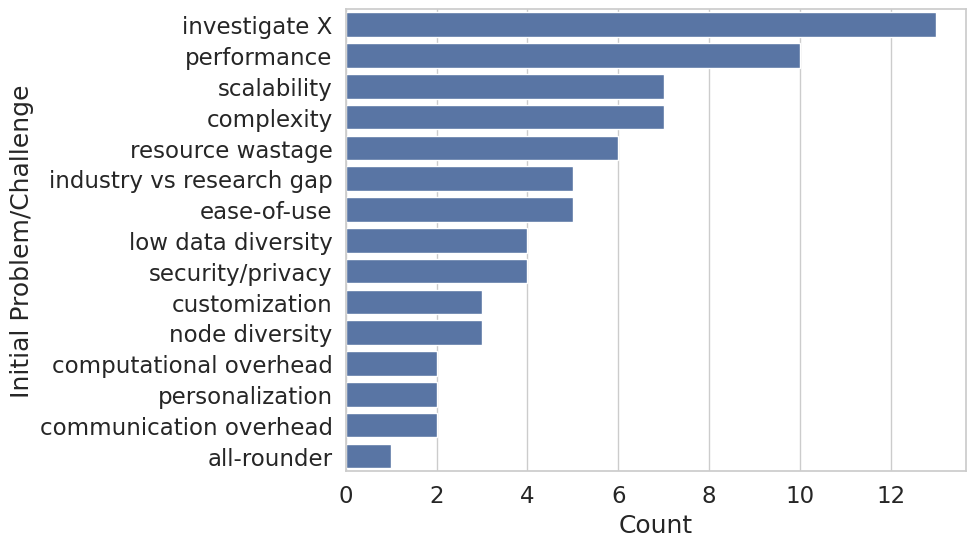
\includegraphics[width=1.0\textwidth]{fl_research_problem_challenge.png}
    \caption{Targeted Problems \& Challenges of FL Papers}
    \label{fig:fl_research_problem_challenge}

    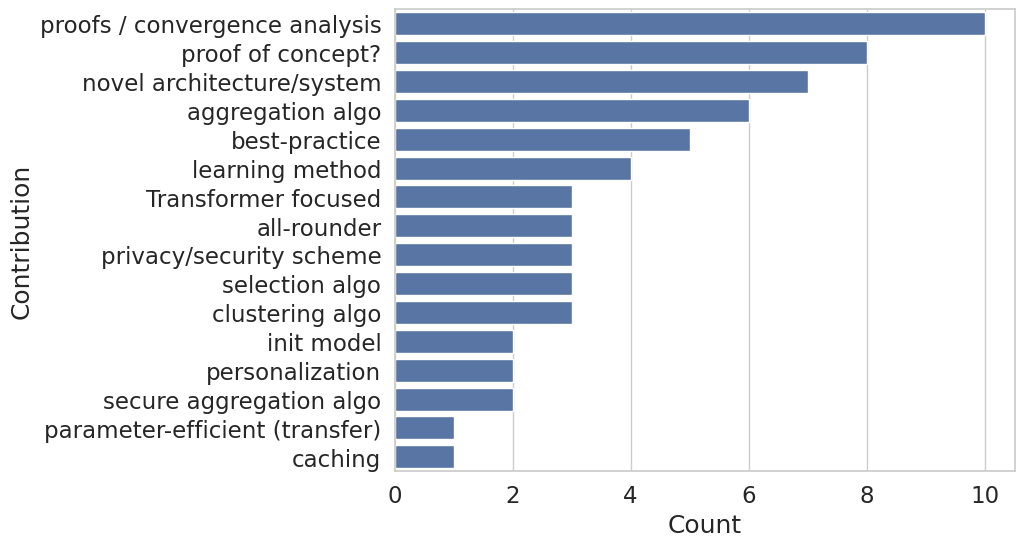
\includegraphics[width=1.0\textwidth]{fl_research_contributions.png}
    \caption{FL Paper Contributions}
    \label{fig:fl_research_contributions}
\end{figure}
\begin{figure}[h]
    \centering
    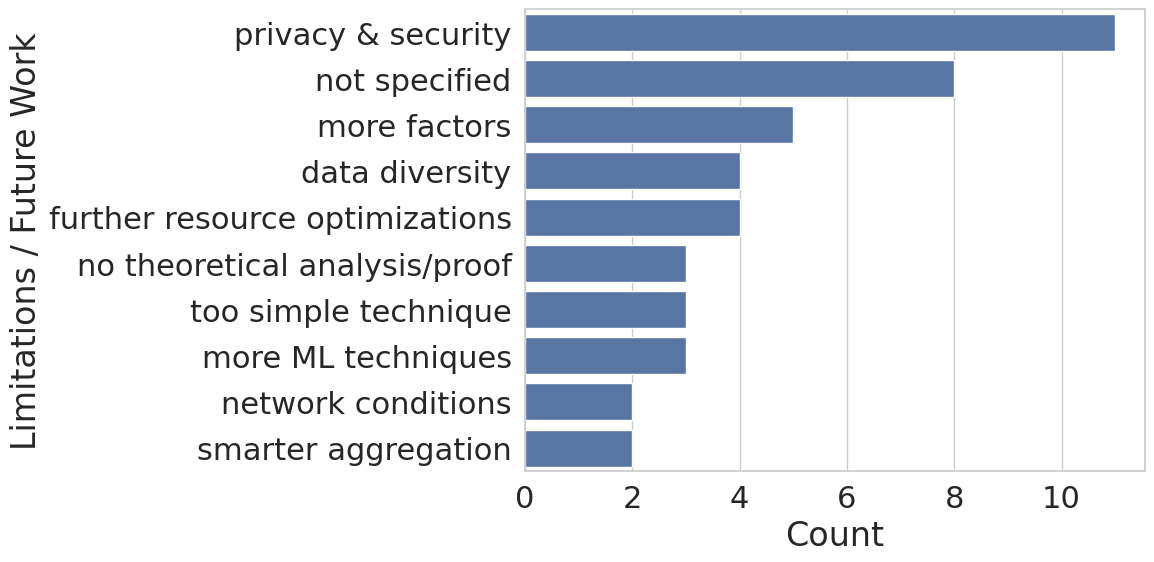
\includegraphics[width=0.9\textwidth]{fl_research_limitations_future_work.png}
    \caption{Limitations \& Future Work of FL Papers}
    \label{fig:fl_research_limitations_future_work}
\end{figure}
